\documentclass[10pt,twocolumn,letterpaper]{article}
\usepackage[letterpaper,top=0.60in,bottom=0.64in,left=0.56in,right=0.56in,columnsep=0.20in]{geometry}
\usepackage{mathptmx}
\usepackage{amsmath,amssymb,amsthm}
\usepackage{booktabs}
\usepackage{tabularx}
\usepackage{graphicx}
\usepackage{xcolor}
\usepackage{hyperref}
\usepackage{caption}
\usepackage{fancyhdr}
\usepackage{microtype}

\renewcommand{\thesection}{\Roman{section}}
\renewcommand{\thesubsection}{\Alph{subsection}}
\renewcommand{\thetable}{\Roman{table}}

\makeatletter
\renewcommand{\section}{\@startsection{section}{1}{\z@}{7pt plus 1.5pt minus 1.5pt}{3pt plus 1pt}{\centering\normalfont\normalsize\scshape}}
\renewcommand{\subsection}{\@startsection{subsection}{2}{\z@}{5.5pt plus 1pt minus 1pt}{1.5pt plus 0.5pt}{\normalfont\normalsize\itshape}}
\makeatother

\setlength{\parskip}{1.5pt plus 0.5pt minus 0.5pt}
\setlength{\parindent}{1em}
\setlength{\textfloatsep}{6pt plus 1.5pt minus 1.5pt}
\setlength{\dbltextfloatsep}{7pt plus 1.5pt minus 1.5pt}
\setlength{\intextsep}{6pt plus 1.5pt minus 1.5pt}
\setlength{\abovecaptionskip}{3pt}
\setlength{\belowcaptionskip}{2pt}
\captionsetup{font=footnotesize,labelfont=bf}
\renewcommand{\arraystretch}{0.92}
\sloppy

\definecolor{ieeeNavy}{RGB}{20,50,92}
\definecolor{ieeeTeal}{RGB}{0,122,120}

\newtheorem{theorem}{Theorem}

\hypersetup{
    colorlinks=true,
    linkcolor=ieeeNavy,
    citecolor=ieeeNavy,
    urlcolor=ieeeTeal,
    pdftitle={NOSIH: A Carbon-Aware, Zero-Trust Neuro-Symbolic Orchestration System},
    pdfauthor={GOKULRAMAN B}
}

\pagestyle{fancy}
\fancyhf{}
\fancyhead[R]{\footnotesize\thepage}
\renewcommand{\headrulewidth}{0pt}

\begin{document}

\twocolumn[{%
\begin{@twocolumnfalse}
\begin{center}
{\fontsize{16.5}{20}\selectfont\textbf{NOSIH: A Carbon-Aware, Zero-Trust Neuro-Symbolic Orchestration System for Energy-Efficient Agentic AI}\par}
\vspace{6pt}
{\normalsize
GOKULRAMAN B\\
\textit{Bachelor of Technology -- Artificial Intelligence and Data Science}\\
\textit{Rajalakshmi Institute of Technology}\\
Chennai, India\\
\texttt{gokulrmn2178@mail.com}
\par}
\vspace{6pt}
\end{center}
\end{@twocolumnfalse}
}]

\noindent\textbf{\textit{Abstract}---Agentic AI systems connect large language models (LLMs) to external Model Context Protocol (MCP) tools, creating a coupled sustainability, reliability, and security problem. GPU-resident models waste active energy on deterministic tasks and draw substantial idle power between bursts, static routers degrade under diurnal grid carbon shifts and distribution drift, and untrusted tool outputs enable indirect prompt injection, schema rug pulls, capability replay, and semantic cache poisoning. We present \textbf{NOSIH}, a unified neuro-symbolic orchestration kernel that couples three planes in a closed loop: zero-trust tool-boundary isolation with RFC~8785 canonicalization, Macaroon capabilities, an Integrity $\times$ Confidentiality provenance semiring, exact-\texttt{Decimal} linear budgets, and Merkle transparency logging (Plane~I); provenance-scoped semantic caching, diurnal carbon-aware primal-dual routing, and online Conformal PID risk control (Plane~II); and deterministic CPU symbolic engines paired with pre-authorized three-state GPU power management and durable replay (Plane~III). On a 240-prompt diurnal benchmark combining physically measured host-CPU execution ($80$ symbolic/RAG queries, Plane~I security, and concurrency) with calibrated neural traces ($160$ queries), NOSIH achieves hybrid experimental estimates of $-75.2\%$ active energy, $-68.7\%$ $\text{CO}_2$, $-63.1\%$ cost, $-67.8\%$ latency, and $-79.35\%$ idle GPU power at $97.50\%$ hybrid task success, blocks $70/70$ tool-boundary attacks ($30/30$ benign utility), and removes $96.9\%$ of Carbon-Denial-of-Wallet emissions and $100.0\%$ of Sleep-Thrashing DoS waste.}

\vspace{3pt}
\noindent\textbf{\textit{Index Terms}---Agentic AI, carbon-aware computing, neuro-symbolic orchestration, zero-trust isolation, Model Context Protocol (MCP), Macaroon capabilities, provenance semirings, online conformal PID, GPU power management.}

\section{Introduction}

\subsection{Motivation: The Agentic Orchestration Trilemma}
Large language models (LLMs) are rapidly shifting from single-turn text generators to autonomous planners inside multi-step agent frameworks such as AutoGen~\cite{wu2024autogen} and MetaGPT~\cite{hong2024metagpt}. Through the Model Context Protocol (MCP)~\cite{gaire2025sok}, these agents read enterprise databases, trigger ERP payouts, and invoke external webhooks. Moving from stateless chat to tool-using execution exposes a tightly coupled \emph{Sustainability--Reliability--Security Trilemma} at the orchestration layer.

On the \emph{sustainability} axis, a single user workflow often fans out into dozens of planning, extraction, and verification calls. Executing deterministic arithmetic, policy retrieval, or structured validation on a $175\text{ W}$ GPU burns orders of magnitude more energy than running a $<5\text{ W}$ CPU symbolic operator~\cite{wan2024neurosymbolic,strubell2019energy,patterson2021carbon}. Compounding this active waste, keeping idle weights pinned in GPU VRAM draws $18\text{--}45\text{ W}$ per tier between bursts, while regional grid carbon intensity swings $2.7\times\text{--}5.9\times$ intraday~\cite{carbonrouter2026}.

On the \emph{security} axis, connecting probabilistic planners to privileged MCP tools with ambient credentials exposes the runtime to indirect prompt injection (IPI), tool-description poisoning, mid-session schema rug pulls, concurrent capability replay, split-payout double-spending, and cross-tenant semantic cache poisoning~\cite{wang2025mcptox,gaire2025sok,wu2026cachepoison}. Prompt-level guardrails cannot reliably prevent adversarial payloads embedded inside vendor emails or remote schemas from hijacking downstream tool calls~\cite{debenedetti2025camel,wang2025mcptox}.

On the \emph{reliability} axis, production workloads are non-stationary: document corpora rotate, model calibration drifts, and inference backends experience transient latency spikes. Static routing thresholds and offline split-conformal calibration lose coverage under distribution shift, either breaching latency and carbon budgets or accepting overconfident errors.

\subsection{Why Decoupled Point Solutions Fail}
Existing research addresses these three axes in isolation, yet assembling independent components leaves structural vulnerabilities at their boundaries. Weight compression~\cite{schwartz2020greenai,han2016deep} shrinks per-token compute offline without altering multi-step agent loops. Carbon-aware batch schedulers~\cite{radovanovic2022carbon,wiesner2021wait} defer jobs across hours, which violates interactive latency targets. Cost-oriented LLM routers such as FrugalGPT~\cite{chen2024frugalgpt} and RouteLLM~\cite{ong2025routellm} ignore live grid carbon intensity, GPU sleep states, and cryptographic tool isolation. Conversely, agent security architectures such as CaMeL~\cite{debenedetti2025camel}, FIDES~\cite{costa2025fides}, and Progent~\cite{shi2025progent} separate control from untrusted data without modeling energy, carbon, semantic caching, or online risk calibration.

In practice, these concerns interact directly: a semantic cache blind to provenance permits cross-tenant poisoning~\cite{wu2026cachepoison}; a carbon-aware router lacking provenance pricing can be tricked by adversarial filler into invoking $175\text{ W}$ GPUs during fossil peaks; and a reactive GPU sleep controller that wakes weights before authorization checks can be drained by rejected probes. Table~\ref{tab:comparison} contrasts existing paradigms against NOSIH across eleven core capabilities.

\subsection{Contributions}
We present \textbf{NOSIH}, a standalone \textbf{Tri-Plane Closed-Loop Neuro-Symbolic Orchestration System} that binds every cache lookup, routing decision, DAG hop, and GPU power transition to shared cryptographic provenance labels and online primal-dual telemetry. Our contributions are:
\begin{itemize}\setlength{\itemsep}{0.6pt}\setlength{\topsep}{2pt}\setlength{\parsep}{0pt}
    \item \textbf{C1 (Unified Tri-Plane Kernel):} A closed-loop kernel uniting Zero-Trust Security (Plane~I), Carbon-Conformal Control (Plane~II), and Durable Execution \& Power Control (Plane~III) across a deterministic seven-stage lifecycle.
    \item \textbf{C2 (Anti-Spoofing Profiling \& Provenance-Scoped Caching):} A sub-millisecond 10D CPU profiler paired with PS-RCSC, a provenance-partitioned BLAS semantic cache featuring cost-aware bypass and conformal admission.
    \item \textbf{C3 (Carbon-Aware Primal-Dual Routing \& Conformal PID):} CA-DPD-LinUCB over deterministic CPU engines and three neural tiers, steered by continuous diurnal carbon $C(t)$ and Dual-Channel Online Conformal PID ($\alpha=0.05$).
    \item \textbf{C4 (CAT-PLM Zero-Trust Reference Monitor):} Non-bypassable enforcement combining strict RFC~8785 JCS, signed boot manifests, offline-attenuable Macaroons with SQLite WAL JTI replay protection, an Integrity $\times$ Confidentiality provenance semiring with exact-\texttt{Decimal} linear budgets, and an RFC~6962/9162 Merkle transparency log.
    \item \textbf{C5 (Predictive Power Control \& Reproducible Evaluation):} Three-state GPU power management (PCS-PMC) with EWMA hysteresis, verified via a 240-prompt 3-seed diurnal benchmark, 7-condition ablation, 100-case security suite, 5-seed shift study, concurrency stress tests, and $46/46$ automated tests.
    \item \textbf{C6 (Irreducible Cross-Plane Primitives):} Three coupled defenses unattainable in decoupled stacks—PCSP ($-96.9\%$ C-DoW $\text{CO}_2$), PA-PCS-PMC ($-100.0\%$ Sleep-Thrashing DoS waste), and CCEC ($O(\log N)$ Scope-2 audit receipts).
\end{itemize}

\begin{table*}[!t]
\centering
\caption{Comparison of Existing Paradigms and NOSIH Across Eleven Architectural Capabilities ($\checkmark$: Supported; P: Partial; $\times$: Not Supported)}
\label{tab:comparison}
\scriptsize
\begin{tabularx}{\textwidth}{Xcccccc}
\toprule
\textbf{Architectural Capability} & \textbf{Green AI}~\cite{schwartz2020greenai,han2016deep} & \textbf{Agentic AI}~\cite{wu2024autogen,hong2024metagpt} & \textbf{Carbon-Aware}~\cite{radovanovic2022carbon,li2025ecoserve} & \textbf{LLM Routers}~\cite{chen2024frugalgpt,ong2025routellm} & \textbf{Agent Security}~\cite{debenedetti2025camel,costa2025fides,shi2025progent} & \textbf{NOSIH (Ours)} \\
\midrule
Dynamic Neuro-Symbolic Routing & $\times$ & P & $\times$ & P & $\times$ & $\checkmark$ \\
Dynamic Diurnal Carbon Optimization & P & $\times$ & $\checkmark$ & $\times$ & $\times$ & $\checkmark$ \\
Predictive Multi-State Sleep (Hysteresis) & P & $\times$ & P & $\times$ & $\times$ & $\checkmark$ \\
Tool-Boundary IPI Isolation / IFC Lattice & $\times$ & $\times$ & $\times$ & $\times$ & $\checkmark$ & $\checkmark$ \\
Cryptographic Capabilities \& Merkle Audit & $\times$ & $\times$ & $\times$ & $\times$ & P & $\checkmark$ \\
Online Conformal Risk Control ($\alpha=0.05$) & $\times$ & $\times$ & $\times$ & $\times$ & $\times$ & $\checkmark$ \\
Provenance-Scoped Semantic Caching & $\times$ & $\times$ & P & P & $\times$ & $\checkmark$ \\
C-DoW Carbon-Security Pricing (PCSP) & $\times$ & $\times$ & $\times$ & $\times$ & $\times$ & $\checkmark$ \\
Cryptographic Carbon Certificates (CCEC) & $\times$ & $\times$ & $\times$ & $\times$ & $\times$ & $\checkmark$ \\
Pre-Auth Sleep-Thrashing Defense (PA-PCS-PMC) & $\times$ & $\times$ & $\times$ & $\times$ & $\times$ & $\checkmark$ \\
Unified Closed-Loop Kernel & $\times$ & $\times$ & $\times$ & $\times$ & $\times$ & $\checkmark$ \\
\bottomrule
\end{tabularx}
\end{table*}

\section{Related Work}

\textbf{Green AI and Neuro-Symbolic Offload.} Strubell et al.~\cite{strubell2019energy}, Schwartz et al.~\cite{schwartz2020greenai}, and Patterson et al.~\cite{patterson2021carbon} established energy and carbon as first-class AI metrics, spurring pruning and quantization~\cite{han2016deep}. Wan et al.~\cite{wan2024neurosymbolic} demonstrated that symbolic arithmetic and structured lookups are memory- and control-flow-bound on GPUs and execute far more efficiently on $<5\text{ W}$ CPUs. NOSIH positions deterministic CPU engines ahead of neural tiers so GPUs activate only when symbolic operators cannot certify an answer.

\textbf{Carbon-Aware Serving and GPU Power Control.} Intraday grid carbon varies $2.7\times\text{--}5.9\times$ within a single balancing area~\cite{carbonrouter2026}. Temporal batch schedulers~\cite{radovanovic2022carbon,wiesner2021wait} shift jobs across hours, whereas online serving frameworks—EcoServe~\cite{li2025ecoserve}, GreenCache~\cite{tian2025greencache}, and GAR~\cite{sheshanarayana2026gar}—adapt routing and caching dynamically. Hardware power controllers such as Patel et al.~\cite{patel2024power}, throttLL'eM~\cite{kakolyris2025throttllem}, and vLLM Sleep Mode~\cite{vllm2025sleep} cut active and idle GPU draw. NOSIH integrates continuous diurnal carbon modeling with an EWMA-hysteresis sleep FSM (PCS-PMC) whose wakeups are strictly gated by pre-authorization.

\textbf{Adaptive Routing, Conformal Control, and Cache Security.} FrugalGPT~\cite{chen2024frugalgpt}, RouterBench~\cite{hu2024routerbench}, and RouteLLM~\cite{ong2025routellm} lower API spend through cascades but assume stationary query distributions. NOSIH pairs discounted linear bandits~\cite{russac2019dlinucb} and primal-dual knapsacks~\cite{agrawal2016lincbwk} with Conformal Risk Control~\cite{angelopoulos2024crc} and Conformal PID~\cite{angelopoulos2023pid} for distribution-free online risk adaptation, while stopping cross-tenant semantic cache poisoning~\cite{wu2026cachepoison} via cryptographic provenance keys.

\textbf{Agentic Security and MCP Isolation.} MCPTox~\cite{wang2025mcptox} and SoK MCP~\cite{gaire2025sok} catalog tool poisoning, schema rug pulls, and confused-deputy exploits in MCP ecosystems. CaMeL~\cite{debenedetti2025camel}, FIDES~\cite{costa2025fides}, and Progent~\cite{shi2025progent} enforce control/data separation inside planners. NOSIH enforces information-flow and capability invariants at both the JSON-RPC~2.0 wire boundary and every DAG hop using RFC~8785 JCS~\cite{rfc8785}, Macaroons~\cite{birgisson2014macaroons}, provenance semirings~\cite{green2007semirings}, and RFC~6962/9162 Merkle logs~\cite{rfc6962,rfc9162}.

\section{The Unified NOSIH Architecture}

\subsection{Tri-Plane Topology and 7-Stage Closed-Loop Lifecycle}
Rather than stacking an external security proxy ahead of an independent LLM router, NOSIH executes as a single closed-loop kernel (\texttt{ZeroTrustKernel}, Fig.~\ref{fig:arch}) in which three planes share cryptographic provenance labels, attenuated capabilities, and live carbon-cost telemetry. Table~\ref{tab:notation} summarizes our notation, and Table~\ref{tab:lifecycle} details the cross-plane ownership and invariants across all seven stages:
\begin{enumerate}\setlength{\itemsep}{0.8pt}\setlength{\topsep}{2pt}\setlength{\parsep}{0pt}
    \item \textbf{Stage 1 — JCS Ingress \& Provenance Binding (Plane~I):} Strict RFC~8785 parsing rejects malformed frames and private/evaluator keys, binding an immutable origin tuple $\tau_0 = (\ell_{\mathcal{I}}, \ell_{\mathcal{C}}, \emptyset)$ directly from the signed boot policy.
    \item \textbf{Stage 2 — 10D Anti-Spoofing CPU Profiling (Plane~II):} A zero-GPU extractor computes ten lexical, structural, symbolic-cue, and Shannon-entropy features $\mathbf{x}_t \in \mathbb{R}^{10}$ in $<0.02\text{ ms}$, neutralizing repetition stuffing and unique-filler escalation.
    \item \textbf{Stage 3 — Provenance-Scoped Semantic Cache (PS-RCSC, Plane~II $\leftrightarrow$ I):} Partitioned by JCS digest $\kappa$ over \texttt{(tenant, corpus\_ver, model\_ver, policy\_epoch, origin\_integrity, schema\_digest)}, untrusted or high-risk ($r_{\text{risk}} \ge 0.50$) queries bypass caching, deterministic CPU workloads take a $0.018\text{ ms}$ cost-aware bypass, and eligible neural queries perform float32 BLAS lookup gated by polarity/numeric guards and Channel-2 Conformal $p$-values.
    \item \textbf{Stage 4 — Carbon- \& Provenance-Aware Dispatch (CA-DPD-LinUCB + PCSP, Plane~II $\leftrightarrow$ I):} On a cache miss, the discounted primal-dual bandit reads diurnal carbon $C(t)$, dual multipliers $\boldsymbol{\mu}_t$, and Plane~I's integrity rank $\iota(x)$ via PCSP to select tier $a_t \in \{T_{0\text{b}}, T_1, T_2, T_3\}$ and emit a typed acyclic DAG $G=(V,E)$.
    \item \textbf{Stage 5 — Static Kahn+IFC Verification \& Macaroon Minting (Planes~III $\leftrightarrow$ I):} Before any GPU or tool executes, Plane~III checks acyclicity (Kahn sort) and static abstract-interpretation IFC (rejecting \texttt{UNTRUSTED} edges into trusted sinks); Plane~I then derives session key $K_{s,u}$ and mints a root \texttt{SPCCE-Macaroon} bound to the canonical plan digest.
    \item \textbf{Stage 6 — Pre-Authorized Async Execution, PA-PCS-PMC \& CCEC Commit (Planes~III $\leftrightarrow$ I):} An \texttt{asyncio} ready-queue runs DAG nodes under hard \texttt{wait\_for} timeouts. Each hop attenuates its Macaroon offline with a 128-bit single-use \texttt{jti}, wakes sleeping GPUs via PA-PCS-PMC \emph{only after} Plane~I verification passes, wraps outputs in \texttt{ProvenanceValue}, journals canonical hashes to SQLite WAL, and commits an RFC~8785 Carbon-Attested Execution Certificate (CCEC) to \texttt{MTLog}.
    \item \textbf{Stage 7 — Dual-Channel Conformal PID \& Dual Feedback (Plane~II):} Channel-1 Conformal PID updates selective risk threshold $\tau_{t+1}^{\text{route}}$, while CA-DPD-LinUCB updates $\mathbf{V}_{t,a}$ and dual prices $\boldsymbol{\mu}_{t+1}$ from observed accuracy, latency, energy, and grid carbon.
\end{enumerate}

\begin{table*}[!t]
\centering
\caption{NOSIH 7-Stage Closed-Loop Lifecycle: Cross-Plane Ownership, Formal Invariants, Complexity, and Prevented Failures}
\label{tab:lifecycle}
\scriptsize
\begin{tabularx}{\textwidth}{clllX}
\toprule
\textbf{Stage} & \textbf{Mechanism} & \textbf{Planes} & \textbf{Complexity / Cost} & \textbf{Architectural Invariant \& Failure Prevented} \\
\midrule
1 & JCS Ingress \& Provenance Binding & I & $O(|q|)$, $<0.05\text{ ms}$ & Rejects duplicate keys, lone surrogates, and private key leakage \\
2 & 10D Anti-Spoofing CPU Profiler & II & $O(|q|)$, $<0.02\text{ ms}$ & Defeats repetition stuffing \& unique-filler denial-of-wallet \\
3 & PS-RCSC Provenance Cache & II $\leftrightarrow$ I & $0.018\text{ ms}$ bypass / $1.8\text{ ms}$ BLAS & Isolates tenants/epochs; stops cross-context cache poisoning \\
4 & CA-DPD-LinUCB + PCSP Pricer & II $\leftrightarrow$ I & $O(Kd^2)$, $<15\,\mu\text{s}$ & Jointly bounds energy, carbon, latency; caps untrusted C-DoW \\
5 & Static Kahn+IFC \& Macaroon Mint & III $\leftrightarrow$ I & $O(|V|+|E|)$, $<0.2\text{ ms}$ & Blocks cyclic/tainted DAGs pre-execution; eliminates self-minting \\
6 & Async DAG, PA-PCS-PMC \& CCEC & III $\leftrightarrow$ I & $O(\log N)$ Merkle & Zero-Joule Sleep-DoS gating, atomic WAL budgets, ESG receipts \\
7 & Conformal PID \& Dual Feedback & II & $O(W)$, $<10\,\mu\text{s}$ & Adapts routing thresholds \& carbon duals under distribution shift \\
\bottomrule
\end{tabularx}
\end{table*}

\begin{table}[!t]
\centering
\caption{Mathematical Notation}
\label{tab:notation}
\scriptsize
\begin{tabularx}{\linewidth}{lX}
\toprule
\textbf{Symbol} & \textbf{Definition} \\
\midrule
$q_t, \mathbf{x}_t$ & Input query at step $t$ and 10D CPU feature vector ($\mathbb{R}^{10}$) \\
$\mathcal{A}$ & Tiers $\{T_{0\text{a}}, T_{0\text{b}}, T_1, T_2, T_3\}$ (Cache, CPU Ops, S/M/L) \\
$C(t)$ & Diurnal grid carbon intensity ($\text{gCO}_2\text{eq/kWh}$) \\
$E(m), L(m)$ & Expected energy ($\text{kWh}$) and latency ($\text{ms}$) of tier $m$ \\
$\mathbf{V}_{t,a}, \boldsymbol{\mu}_t$ & Discounted Gram matrix and primal-dual multipliers \\
$\alpha, \tau_t^{\text{route}}$ & Target risk ($0.05$) and Conformal PID threshold \\
$\kappa, \tau_t^{\text{cache}}$ & JCS provenance cache key and cache conformal threshold \\
$\mathcal{L}=\mathcal{I}\times\mathcal{C}$ & Integrity $\times$ Confidentiality product lattice ($\oplus,\otimes$) \\
$C_k, \text{jti}, B_w$ & Attenuated Macaroon, WAL nonce, and exact-\texttt{Decimal} budget \\
$s_m, \tau_{\text{be}}$ & Tier power state and hysteresis break-even idle threshold \\
\bottomrule
\end{tabularx}
\end{table}

\begin{figure*}[!t]
\centering
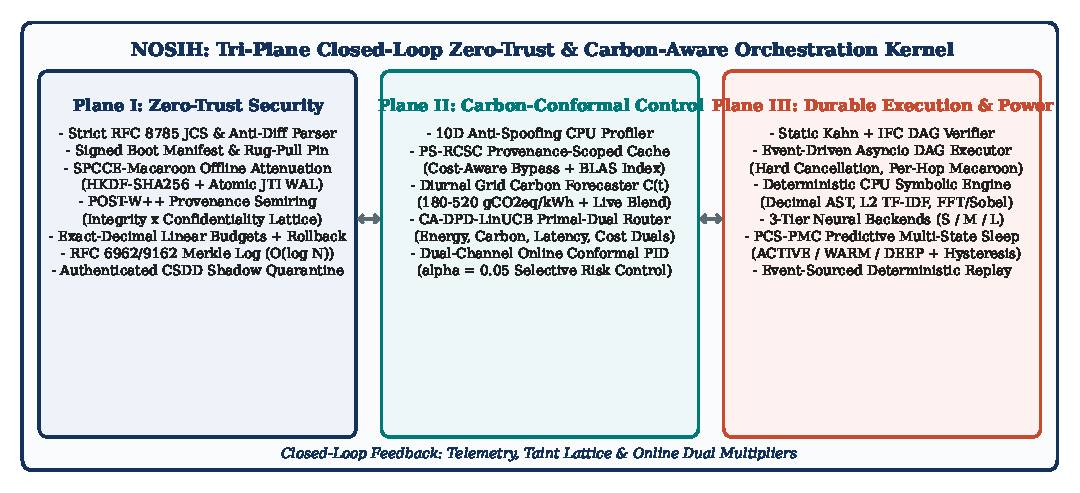
\includegraphics[width=0.90\textwidth]{figures/fig1_architecture.pdf}
\caption{NOSIH Tri-Plane Closed-Loop Architecture unifying CAT-PLM zero-trust security (Plane~I), carbon-conformal routing and provenance-scoped caching (Plane~II), and neuro-symbolic durable execution with PCS-PMC power control (Plane~III).}
\label{fig:arch}
\end{figure*}

\subsection{Plane~I: Threat Model and CAT-PLM Zero-Trust Kernel}
\textbf{Trusted Computing Base \& Adversary.} The TCB comprises the NOSIH kernel modules (\texttt{jcs\_v3}, \texttt{proxy\_v3}, \texttt{spcce\_v3}, \texttt{postw\_v3}, \texttt{merkle\_log}, \texttt{shadow\_v3}), the out-of-band signed tool manifest, and the SQLite WAL ledger. All LLM planners, retrieved documents, remote MCP servers, and network frames are untrusted: an adversary may inject prompts via retrieved text, mutate tool schemas at boot or mid-session (rug pulls), craft duplicate-key JSON frames, replay capabilities across concurrent threads, split payouts to breach invoice ceilings, exfiltrate ERP secrets via Base64/hex/chunking, or truncate audit logs.

\textbf{Strict RFC~8785 JCS \& Signed Manifest Pinning.} Every JSON-RPC~2.0 frame passes an anti-differential parser that rejects duplicate keys, non-finite floats, integers outside $\pm(2^{53}-1)$, and lone UTF-16 surrogates prior to ECMAScript canonicalization~\cite{rfc8785}. At boot, an out-of-band HMAC-SHA256 signed manifest pins every permitted tool digest (removing Day-0 TOFU); every subsequent \texttt{tools/list} and \texttt{tools/call} re-checks digests, stripping mutated tools and logging \texttt{RUG\_PULL\_DETECTED}.

\textbf{Offline-Attenuable Capabilities (\texttt{SPCCE-Macaroon}).} Root secrets require at least 256 bits per \texttt{key\_id} with no default fallback. Per-session keys derive via RFC~5869 HKDF-SHA256:
\begin{equation}
\begin{aligned}
K_{s,u} = \text{HKDF-SHA256}\Big(&K_{\text{root}}[\text{kid}],\; u \parallel \texttt{":"} \parallel s,\\
&\texttt{"NOSIH-CAP-ROOT"}\Big).
\end{aligned}
\end{equation}
Starting from root tag $\sigma_0 = \text{HMAC-SHA256}(K_{s,u}, \texttt{ROOT}\parallel\text{JCS}(\text{header}))$, parent DAG nodes attenuate capabilities offline for child hop $v_{k+1}$ without holding $K_{s,u}$ by chaining caveats $c_{k+1}$ (tool allowlists, exact-\texttt{Decimal} ceilings, hop/schema pins, TTLs, and 128-bit CSPRNG \texttt{jti}s):
\begin{equation}
\sigma_{k+1} = \text{HMAC-SHA256}\!\left(\sigma_k,\; \texttt{CAV} \parallel \text{JCS}(c_{k+1})\right).
\end{equation}
Each tool call consumes its \texttt{jti} atomically inside a SQLite WAL \texttt{BEGIN IMMEDIATE} transaction with TTL pruning, permitting out-of-order concurrent DAG branches with zero self-minting.

\textbf{Provenance Semiring (\texttt{POST-W++}) \& Linear Budgets.} Every runtime value carries $\tau(v) = (\ell_{\mathcal{I}}, \ell_{\mathcal{C}}, W, h_{\text{deriv}})$ over $\mathcal{L} = \mathcal{I} \times \mathcal{C}$, where integrity is ordered $\text{HUMAN}(0) \sqsubset \text{GOV}(1) \sqsubset \text{ERP}(2) \sqsubset \text{POLICY}(3) \sqsubset \text{USER}(4) \sqsubset \text{DET}(5) \sqsubset \text{UNTRUSTED}(6)$ ($\sqcup_{\mathcal{I}}=\max$) and confidentiality pairs sensitivity tier with reader intersection $(t_1,R_1)\sqcup_{\mathcal{C}}(t_2,R_2)=(\max(t_1,t_2), R_1\cap R_2)$. Identity $\mathbf{1}=(\text{HUMAN}(0),(\text{PUBLIC},\mathcal{U}),\emptyset)$ and absorber $\mathbf{0}=(\text{UNTRUSTED}(6),(\text{RESTRICTED},\emptyset),\emptyset)$ guarantee monotonic taint propagation. Origin labels come solely from the signed policy map. Financial witnesses maintain exact-\texttt{Decimal} linear budgets decremented atomically in SQLite WAL with failure rollback; egress webhooks enforce $\ell_{\mathcal{C}} \sqsubseteq_{\mathcal{C}} \text{clear}(e)$ alongside plaintext, Base64, hex, chunked, and high-entropy exfiltration scans.

\textbf{Merkle Transparency (\texttt{MTLog}) \& Shadow Quarantine.} Every audit record appends atomically to an RFC~6962/9162 binary Merkle tree with domain-separated leaf ($\texttt{0x00}$) and interior ($\texttt{0x01}$) SHA-256 digests, issuing signed Tree Heads (STHs) and $O(\log N)$ inclusion and consistency proofs. Blocked sink calls divert to \texttt{CSDDShadowSink}, returning MAC-authenticated, Merkle-anchored quarantine receipts.

\begin{theorem}[Non-Escalation \& Monotonic Attenuation]
Assume EUF-CMA security of HMAC-SHA256 ($\lambda=256$ bits) and SHA-256 collision resistance. Given a valid capability $C_k = (\text{header}, [c_1,\dots,c_k], \sigma_k)$, no PPT adversary without $K_{s,u}$ can forge an accepted $C'$ authorizing $r \notin \bigcap_{i=1}^k \mathcal{A}(c_i)$ with probability exceeding $\text{Adv}^{\text{EUF-CMA}}_{\text{HMAC}}(\lambda) + 2^{-\lambda}$.
\end{theorem}
\noindent\textit{Proof Sketch.} Removing or altering any caveat $c_j$ ($j\le k$) or \texttt{header} requires forging an HMAC under unknown $\sigma_{j-1}$ or colliding SHA-256; appending caveats strictly shrinks $\bigcap \mathcal{A}(c_i)$. Full proof in \texttt{docs/FORMAL\_PROOFS.md}. \hfill$\square$

\begin{theorem}[Concurrent Replay \& Linear Budget Soundness]
Assume SQLite WAL \texttt{BEGIN IMMEDIATE} serialization, durable storage, and 128-bit CSPRNG nonces. Across any $T$ concurrent threads: (a) at most one invocation per unique \texttt{jti} executes; and (b) for any financial witness $w$ with exact-\texttt{Decimal} budget $B_w$, cumulative payouts satisfy $\sum_j a_j \le B_w$.
\end{theorem}
\noindent\textit{Proof Sketch.} \texttt{BEGIN IMMEDIATE} acquires a \texttt{RESERVED} write lock before reading, serializing \texttt{PRIMARY KEY (jti)} inserts and inductive exact-\texttt{Decimal} updates $0 \le \text{rem}_t = B_w - \sum_{j \le t} a_j$ (see \texttt{docs/FORMAL\_PROOFS.md}). \hfill$\square$

\begin{theorem}[Multi-Hop IFC Soundness \& Tamper Evidence]
Assume an acyclic DAG $G=(V,E)$, SHA-256 collision resistance, and \texttt{0x00}/\texttt{0x01} domain separation. Any \texttt{UNTRUSTED} ancestor forces $\ell_{\mathcal{I}}(u)=\text{UNTRUSTED}$ (blocking trusted sinks), any ancestor with $\ell_{\mathcal{C}}(v) \not\sqsubseteq_{\mathcal{C}} \text{clear}(e)$ blocks egress $e$, and modifying or truncating any leaf $i < m$ fails \texttt{MTLog} verification against witnessed $\text{STH}_m$ in $O(\log N)$ time.
\end{theorem}
\noindent\textit{Proof Sketch.} Follows by topological induction from absorptivity of $\sqcup_{\mathcal{I}},\sqcup_{\mathcal{C}}$ and collision reduction at the lowest differing Merkle node (\texttt{docs/FORMAL\_PROOFS.md}). \hfill$\square$

\subsection{Plane~II: Carbon-Conformal Control Plane}
\textbf{Anti-Spoofing Profiler \& PS-RCSC.} The 10D CPU profiler combines normalized length, symbolic cues, risk density, lexical uniqueness, and token/character Shannon entropy, flagging both repetition stuffing ($n>15 \land u<0.55$) and unique-filler denial-of-wallet probes ($n>25 \land u>0.85 \land \text{risk\_density}<0.06$). PS-RCSC isolates entries by provenance digest $\kappa$, serves exact matches in $O(1)$, skips vector lookup when predicted CPU symbolic latency is below cache overhead, and gates float32 BLAS hits on polarity/numeric guards and Channel-2 Conformal $p$-values.

\textbf{Diurnal Carbon Forecasting \& CA-DPD-LinUCB.} NOSIH models continuous diurnal grid carbon intensity $C(t) \in [180, 520]\text{ gCO}_2\text{eq/kWh}$ (Fig.~\ref{fig:workflow}a) as a solar-trough / evening-peak prior plus an Ornstein-Uhlenbeck residual blended with live telemetry via $w(\Delta t)=e^{-\Delta t/900}$:
\begin{equation}
\begin{aligned}
C_{\text{det}}(h) = 355 &- 175 e^{-\frac{(h-13)^2}{2(2.6)^2}} + 165 e^{-\frac{(h-19.5)^2}{2(2.1)^2}}\\
&+ 20\cos\!\left(\tfrac{2\pi(h-2.5)}{24}\right).
\end{aligned}
\end{equation}
CA-DPD-LinUCB maintains exponentially discounted Gram matrices $\mathbf{V}_{t,a} = \gamma \mathbf{V}_{t-1,a} + (1-\gamma)\lambda\mathbf{I} + \mathbf{x}_t\mathbf{x}_t^\top\mathbb{I}\{a_t=a\}$ and dispatches
\begin{equation}
a_t = \arg\max_{a \in \mathcal{A}_t}\left\{\text{UCB}_{t,a}^r(\mathbf{x}_t) - \sum_{m=1}^{M}\mu_t^{(m)}\!\left(\text{LCB}_{t,a}^{(m)}(\mathbf{x}_t) - b^{(m)}\right)\right\},
\end{equation}
updating dual multipliers $\mu_{t+1}^{(m)} = \Pi_{[0,\mu_{\max}]}(\mu_t^{(m)} + \eta_\mu(c_t^{(m)} - b^{(m)}))$ over energy, carbon ($\hat{E}\cdot C(t)$), and latency budgets. Online Conformal PID updates selective risk threshold $\tau_t^{\text{route}}$ via
\begin{equation}
\begin{aligned}
\tau_{t+1}^{\text{route}} = \Pi_{[\tau_{\min}, \tau_{\max}]}\!\Big(&\tau_t^{\text{route}} + \eta(\alpha - \ell_t)\\
&+ k_I \tanh\!\Big(\tfrac{1}{5}\sum_{j=t-W}^{t}(\alpha - \ell_j)\Big)\Big).
\end{aligned}
\end{equation}

\begin{theorem}[Dynamic Regret, Feasibility \& Finite-Sample Risk Control]
Assume bounded contexts $\|x_{t,a}\|_2 \le L$, parameters $\|\theta_{t,a}\|_2 \le S$ with variation budget $\sum_{t=1}^{T-1}\|\theta_{t+1,a}-\theta_{t,a}\|_2 \le B_T$, Slater slack $\rho > 0$, and bounded scores $s_t \in [0,1]$. Setting $\gamma = 1 - (B_T/(dT))^{2/3}$ and $\eta_\mu = O(T^{-1/2})$, CA-DPD-LinUCB achieves dynamic regret $\widetilde{\mathcal{O}}(d^{2/3} B_T^{1/3} T^{2/3} + \rho^{-1}\sqrt{MT})$ and sublinear constraint violation~\cite{russac2019dlinucb,agrawal2016lincbwk}. Under arbitrary distribution shift, the proportional P-channel ($k_I=0$) satisfies $|\frac{1}{T}\sum_{t=1}^T \text{err}_t - \alpha| \le (q_{\max}-q_{\min}+\eta)/(\eta T)$, while adding the bounded nonlinear integral term $k_I\tanh(\cdot)$ accelerates post-shift recovery within a bounded $O(k_I/\eta)$ perturbation~\cite{angelopoulos2023pid}.
\end{theorem}
\noindent\textit{Proof Sketch.} Decomposing Lagrangian regret separates discounted contextual estimation error $\widetilde{\mathcal{O}}(d^{2/3} B_T^{1/3} T^{2/3})$ from dual OGD regret $\widetilde{\mathcal{O}}(\rho^{-1}\sqrt{MT})$ over $M$ constraints. Telescoping $q_{t+1}-q_t = \eta(\text{err}_t-\alpha)$ over $t=1\dots T$ with $|q_{T+1}-q_1| \le q_{\max}-q_{\min}+\eta$ yields the $O(1/(\eta T))$ distribution-free bound (full derivation in \texttt{docs/FORMAL\_PROOFS.md}). \hfill$\square$

\begin{figure}[!t]
\centering
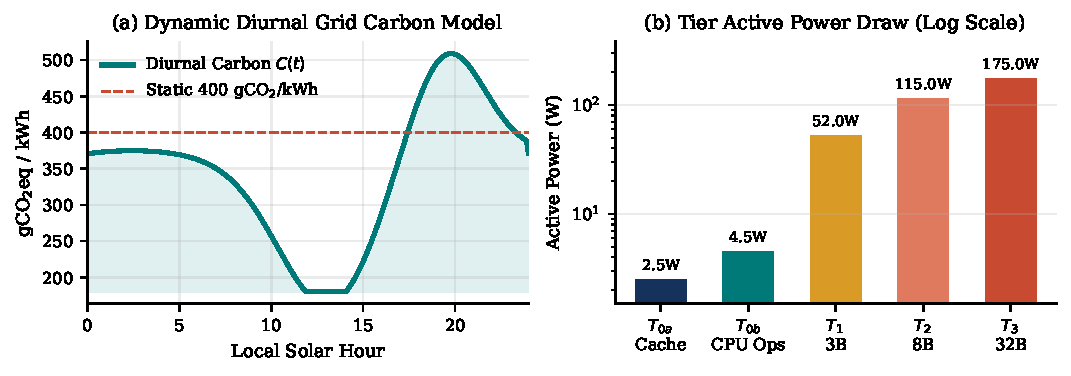
\includegraphics[width=0.96\linewidth]{figures/fig2_workflow.pdf}
\caption{(a) Diurnal grid carbon curve $C(t) \in [180, 520]\text{ gCO}_2\text{eq/kWh}$ vs.\ static $400\text{ gCO}_2/\text{kWh}$; (b) Active power draw across NOSIH's five execution tiers (log scale).}
\label{fig:workflow}
\end{figure}

\subsection{Plane~III: Durable Execution, Power Control \& Complexity}
\textbf{Async DAG Runtime \& Replay.} Plane~III executes an event-driven \texttt{asyncio} ready-queue with per-node \texttt{wait\_for} cancellation across deterministic CPU engines (\texttt{SafeDecimalAST}, L2 TF-IDF RAG, 1024-pt FFT/Sobel) and a 3-state circuit-breaker provider chain (\texttt{CLOSED}/\texttt{OPEN}/\texttt{HALF\_OPEN}). Canonical node hashes commit to a SQLite WAL \texttt{JournalStore} supporting \texttt{RECORD}, bit-identical \texttt{REPLAY}, and \texttt{COUNTERFACTUAL\_DIFF}.

\textbf{Predictive Multi-State Power Control (PCS-PMC).} Each neural tier $m \in \{T_1, T_2, T_3\}$ transitions between \texttt{ACTIVE} ($18\text{--}45\text{ W}$ idle VRAM), \texttt{WARM\_STANDBY} ($8\text{--}18\text{ W}$, $100\text{--}180\text{ ms}$ wake), and \texttt{DEEP\_SLEEP} ($2.5\text{ W}$ RAM-paged, $0.85\text{--}1.40\text{ s}$ wake). Demotion $a\to b$ triggers once idle duration exceeds
\begin{equation}
\tau_{\text{be}}(m, a\to b) = \frac{E_{\text{trans}}(m, a\to b) + E_{\text{wake}}(m, b\to\texttt{ACT})}{P_{\text{idle}}(m, a) - P_{\text{idle}}(m, b)},
\end{equation}
scaled by $H_m = \eta_{\text{down}}(1 + \kappa\min(\text{CV}_m, 2.0))$ from an EWMA inter-arrival estimator with thrash-rate damping. Per-query kernel overhead remains $O(|q|)$ for profiling, $O(Kd^2)$ for routing ($d=10, K=6$, $<15\,\mu\text{s}$), $O(|V|+|E|)$ for static IFC, and $O(\log N)$ for \texttt{MTLog} proofs.

\subsection{Three Irreducible Cross-Plane Primitives}
Placing a standalone security proxy in front of an independent carbon router cannot reproduce three primitives that share live state across all three planes:
\begin{enumerate}\setlength{\itemsep}{0.6pt}\setlength{\topsep}{2pt}\setlength{\parsep}{0pt}
    \item \textbf{Provenance-Coupled Carbon-Security Pricing (PCSP):} Security-blind carbon routers~\cite{sheshanarayana2026gar,carbonrouter2026} are exposed to \emph{Carbon-Denial-of-Wallet (C-DoW)}, where untrusted text mimics complex prompts during fossil peaks to force $175\text{ W}$ GPUs. PCSP injects $\Phi_{\text{PCSP}}(\iota, a, C(t)) = \lambda_{\text{sec}}(\iota/6)(P_a/P_{T_3})(C(t)/C_{\text{ref}})$ into Plane~II's Lagrangian, capping unauthenticated \texttt{UNTRUSTED} traffic at $T_1$ (or $T_{0\text{b}}$) and tightening its risk budget to $\alpha_{\text{eff}}=0.025$.
    \item \textbf{Authorization-Gated \& Carbon-Modulated Sleep (PA-PCS-PMC):} Reactive sleep controllers~\cite{vllm2025sleep} wake GPUs before authorization completes, enabling \emph{Sleep-Thrashing DoS}. PA-PCS-PMC executes Plane~I's $<4\text{ ms}$ Macaroon/IFC check prior to wakeup ($0.0\text{ J}$ wasted on rejected hops) and scales idle hysteresis by $M_C(t)=\operatorname{clip}(C_{\text{ref}}/C(t), 0.65, 1.35)$.
    \item \textbf{Cryptographic Carbon-Attested Execution Certificates (CCEC):} Every execution commits \texttt{(tier, energy\_kwh, grid\_carbon, co2\_g, accounting\_mode, hw\_digest)} as an RFC~8785 leaf in \texttt{MTLog}, providing $O(\log N)$ Scope-2 ESG proofs while rejecting simulated traces spoofed as hardware wattmeter telemetry.
\end{enumerate}

\begin{theorem}[Cross-Plane Non-Decomposability \& C-DoW Bound]
Assume a decoupled stack $(R,S,P)$ where router $R$ lacks Plane~I provenance $\iota(x)$ and sleep controller $S$ wakes $T_3$ before proxy $P$ checks authorization. Against $K$ unauthenticated untrusted prompts during fossil peak $C_{\max}$, $(R,S,P)$ incurs worst-case energy $K(E_{T_3}+E_{\text{wake}})$. Under NOSIH's coupled PCSP + PA-PCS-PMC invariants, unauthorized hops incur $0.0\text{ J}$ wakeup energy, unauthenticated untrusted prompts are bounded by $K E_{T_1}$ (or $K E_{T_{0\text{b}}}$), and every footprint is committed in $O(\log N)$ CCEC proofs.
\end{theorem}
\noindent\textit{Proof Sketch.} Because $S$ precedes $P$ in $(R,S,P)$, every rejected probe wastes $E_{\text{wake}}(T_3)$, whereas NOSIH's \texttt{on\_authorized\_request\_arrival} gates wakeups on Plane~I verification ($0\text{ J}$ waste). Simultaneously, PCSP caps unauthenticated $\iota=\texttt{UNTRUSTED}$ requests at $T_1$/$T_{0\text{b}}$, bounding active energy by $K E_{T_1}$ (full proof in \texttt{docs/FORMAL\_PROOFS.md}). \hfill$\square$

\subsection{Worked Trace: Benign vs.\ Attacked Invoice Workflow}
Consider an enterprise agent settling a vendor invoice during an evening fossil peak ($C(t)=490\text{ gCO}_2/\text{kWh}$). In the \emph{benign} flow, \texttt{get\_vendor\_invoice} returns \texttt{approved\_amount\_inr} labeled $\ell_{\mathcal{I}}=\text{ERP}(2)$ with linear SQLite WAL budget $B_w=\text{INR }50{,}000$. Stage~4 dispatches deterministic GST arithmetic to $T_{0\text{b}}$ ($4.5\text{ W}$, $3.5\text{ ms}$), Stage~5 verifies the acyclic DAG and mints an attenuated Macaroon, and Stage~6 executes \texttt{execute\_neft\_payout} inside \texttt{BEGIN IMMEDIATE} while committing a CCEC receipt to \texttt{MTLog}. Now suppose an \emph{adversary} embeds hidden instructions in \texttt{read\_vendor\_email} ($\ell_{\mathcal{I}}=\text{UNTRUSTED}(6)$) attempting to (a) escalate a complex-looking prompt onto a sleeping $175\text{ W}$ $T_3$ GPU and (b) double-spend or divert the payout. PCSP caps the untrusted prompt at $T_1$/$T_{0\text{b}}$ (blocking C-DoW), PA-PCS-PMC refuses to wake the sleeping $T_3$ GPU when Macaroon/IFC checks fail ($0.0\text{ J}$ wasted), the provenance semiring propagates $\text{ERP}(2)\sqcup_{\mathcal{I}}\text{UNTRUSTED}(6)=\text{UNTRUSTED}(6)$ to quarantine the tainted payout in \texttt{CSDDShadowSink}, and \texttt{MTLog} records the tamper-evident audit leaf.

\section{Experimental Evaluation}

\subsection{Setup, Measurement Boundary, and Carbon Validation}
All experiments are deterministic and reproducible via \texttt{run\_all\_tests.py}, \texttt{run\_nosih\_evaluation.py}, and \texttt{verify\_nosih\_claims.py}. An automated probe (\texttt{hardware\_probe.py}) records Linux \texttt{x86\_64}, Python 3.11.2, \texttt{rapl\_available=false}, and \texttt{nvml\_available=false}. Every record in \texttt{raw\_measurements.jsonl} explicitly separates physically measured host-CPU telemetry from calibrated neural simulation: Plane~I cryptography, JCS parsing, SQLite WAL races, Merkle proofs, async concurrency throughput, and the $80$ CPU symbolic math/RAG queries are \emph{physically measured} on host CPU with exact ground-truth verification (\texttt{eval\_judge=EXACT\_DETERMINISTIC}, $80/80$ exact). Because physical GPUs and NVML/RAPL counters are absent in our container, the $160$ neural queries across $T_1$ 3B ($52\text{ W}$, $\$0.10/\text{M}$), $T_2$ 8B ($115\text{ W}$, $\$0.25/\text{M}$), and $T_3$ 32B ($175\text{ W}$, $\$0.85/\text{M}$)—alongside CPU tiers $T_{0\text{a}}$ Cache ($2.5\text{ W}$, $\$0$) and $T_{0\text{b}}$ Symbolic ($4.5\text{ W}$, $\$0$)—are transparently tagged \texttt{HYBRID\_CPU\_TDP} and \texttt{CALIBRATED\_TRACE\_SIM} ($\phi_{\text{phase}}=0.85$, PUE $=1.0$, $\$0.12/\text{kWh}$) with a calibrated Bernoulli accuracy matrix (\texttt{eval\_judge=CALIBRATED\_BERNOULLI\_SIM}) modeling nominal \texttt{qwen2.5-3b-q4}, \texttt{llama3.1-8b-q4}, and \texttt{qwen2.5-32b-q4} tiers; \texttt{experiments/run\_hardware\_validation.py} is provided for live NVML/RAPL/Ollama deployment.

We evaluate a 240-prompt six-category benchmark (40 each: Symbolic Math/AST, Policy RAG, Simple Factual, Medium Analytical/Coding, Complex Multi-Step, and Ambiguous/Cacheable) across 3 fixed seeds ($\{42,101,202\}$) over a 12-hour diurnal window (09:00--21:00). We compare \textbf{Full NOSIH} against (1) a \textbf{Static Large Baseline} ($T_3$ always active) and (2) a \textbf{Fixed-Threshold Energy-Only Router} (static tier dispatch without symbolic offload, PS-RCSC, or carbon duals, using a fixed $10\text{ s}$ sleep timeout), reporting two-tailed paired Wilcoxon tests ($n=240$, 95\% CI), Rank-Biserial effect sizes ($r_{\text{rb}}$), and 95\% Wilson CIs. To validate diurnal carbon tracking independently of live grid APIs, we tested the forecaster on a held-out $168\text{-h}$ synthetic diurnal+OU trace: the deterministic prior attains $11.37\text{ gCO}_2/\text{kWh}$ MAE ($14.76$ RMSE, $3.63\%$ MAPE), 5-min blending reduces MAE to $4.10$ ($5.33$ RMSE), and 60-min stale fallback holds $14.34$ RMSE.

\subsection{Primary Results, Multimodal Latency, and Stability}
Tables~\ref{tab:primary}--\ref{tab:routing} and Figs.~\ref{fig:ec}--\ref{fig:rp} report end-to-end performance. Relative to Static Large, NOSIH lowers active energy by $75.2\%$ ($0.022479$ to $0.005567\text{ kWh}$, $p=1.26\times 10^{-38}$, $r_{\text{rb}}=0.9678$), $\text{CO}_2$ by $68.7\%$ ($6.9487$ to $2.1728\text{ g}$, $p=1.43\times 10^{-37}$), cost by $63.1\%$ ($\$0.067297$ to $\$0.024826$, $p=7.86\times 10^{-39}$), and latency by $67.8\%$ ($2200.2$ to $707.6\text{ ms}$, $p=2.69\times 10^{-37}$). Offloading $50.0\%$ of traffic to $<5\text{ W}$ CPU paths ($64$ cache hits, $56$ symbolic executions) and dispatching $35/50/35$ to $T_1/T_2/T_3$ lifts task success to $97.50\%$ (vs.\ $97.08\%$ Static Large and $90.83\%$ Fixed-Threshold), cutting energy per successful goal by $75.3\%$ ($0.09648$ to $0.02379\text{ Wh}$). Over the Fixed-Threshold Router, NOSIH saves an additional $18.5\%$ energy ($p=1.15\times 10^{-13}$) and $18.2\%$ $\text{CO}_2$ ($p=2.36\times 10^{-12}$), while PCS-PMC reduces GPU wakeups by $27.7\%$ ($68$ vs.\ $94$) and cuts idle GPU power by $79.35\%$ ($33.6677\text{ Wh}$ net saved, $257.8\text{ ms}$ average wake).

NOSIH's latency SD ($899.6\text{ ms}$) exceeds its mean ($707.6\text{ ms}$) because heterogeneous dispatch is intentionally multimodal: half of all queries finish on CPU in $1.8\text{ ms}$ ($T_{0\text{a}}$) or $3.5\text{ ms}$ ($T_{0\text{b}}$), yielding a median (P50) of $169.8\text{ ms}$ (IQR $1280.3\text{ ms}$), whereas neural tiers $T_1$ ($574.4\text{ ms}$ mean), $T_2$ ($1312.9\text{ ms}$), and $T_3$ ($2393.5\text{ ms}$) plus occasional \texttt{DEEP\_SLEEP} wakeups ($1.4\text{ s}$) place P95 at $2549.2\text{ ms}$ and P99 at $2878.7\text{ ms}$. Across seeds $\{42,101,202\}$, reductions remain tightly clustered at $-75.18\%\pm 0.55\%$ energy, $-68.36\%\pm 0.74\%$ $\text{CO}_2$, $-63.11\%\pm 0.02\%$ cost, and $-67.98\%\pm 0.56\%$ latency.

\begin{table*}[!t]
\centering
\caption{Primary Results ($n=240$, Seed 42; Mean $\pm$ 95\% CI, Paired Wilcoxon Test \& Rank-Biserial $r_{\text{rb}}$ vs.\ Static Large)}
\label{tab:primary}
\scriptsize
\begin{tabularx}{\textwidth}{lcccccc}
\toprule
\textbf{Metric} & \textbf{Static Large} & \textbf{Fixed-Thresh.\ Router} & \textbf{Full NOSIH (Ours)} & $\boldsymbol{\Delta}$ vs.\ Static & $\boldsymbol{\Delta}$ vs.\ Fixed & $\boldsymbol{p}$ / $\boldsymbol{r_{\text{rb}}}$ \\
\midrule
Latency (ms) & $2200.2 \pm 39.7$ & $987.4 \pm 87.4$ & $707.6 \pm 113.8$ & $-67.8\%$ & $-28.3\%$ & $<10^{-36}$ / $0.9502$ \\
Energy/q (kWh) & $9.37\text{e-}5 \pm 1.69\text{e-}6$ & $2.85\text{e-}5$ & $2.32\text{e-}5 \pm 4.49\text{e-}6$ & $-75.2\%$ & $-18.5\%$ & $<10^{-37}$ / $0.9678$ \\
$\text{CO}_2$/q (g) & $0.0290 \pm 0.0016$ & $0.0111$ & $0.0091 \pm 0.0019$ & $-68.7\%$ & $-18.2\%$ & $<10^{-36}$ / $0.9539$ \\
Cost/q (USD) & $2.80\text{e-}4 \pm 1.62\text{e-}5$ & $1.26\text{e-}4$ & $1.03\text{e-}4 \pm 2.34\text{e-}5$ & $-63.1\%$ & $-17.7\%$ & $<10^{-38}$ / $0.9705$ \\
\midrule
Total Energy (kWh) & $0.022479$ & $0.006830$ & $0.005567$ & $-75.2\%$ & $-18.5\%$ & $p=1.15\times 10^{-13}$ (vs.\ Fix.) \\
Total $\text{CO}_2$ (g) & $6.9487$ & $2.6549$ & $2.1728$ & $-68.7\%$ & $-18.2\%$ & $p=2.36\times 10^{-12}$ (vs.\ Fix.) \\
Total Cost (USD) & $0.067297$ & $0.030170$ & $0.024826$ & $-63.1\%$ & $-17.7\%$ & --- \\
Task Success Rate & $97.08\%$ & $90.83\%$ & $\mathbf{97.50\%}$ & $+0.42\text{ pp}$ & $+6.67\text{ pp}$ & --- \\
Energy / Success (Wh) & $0.09648$ & $0.03133$ & $\mathbf{0.02379}$ & $-75.3\%$ & $-24.1\%$ & --- \\
$\text{CO}_2$ / Success (mg) & $29.823$ & $12.179$ & $\mathbf{9.285}$ & $-68.9\%$ & $-23.8\%$ & --- \\
Cost / Success (USD) & $\$0.000289$ & $\$0.000138$ & $\mathbf{\$0.000106}$ & $-63.3\%$ & $-23.2\%$ & --- \\
Idle GPU Power Cut & $0.0\%$ & $69.30\%$ ($94$ wakes) & $\mathbf{79.35\%}$ ($68$ wakes) & $-79.35\%$ & $+10.05\text{ pp}$ & $33.6677\text{ Wh}$ net saved \\
\bottomrule
\end{tabularx}
\end{table*}

\begin{table}[!t]
\centering
\caption{Per-Metric Variability (Mean $\pm$ SD, $n=240$) and 3-Seed Stability}
\label{tab:variability}
\scriptsize
\begin{tabular}{@{}lcc@{}}
\toprule
\textbf{Metric} & \textbf{Static Large} & \textbf{Full NOSIH} \\
\midrule
Latency (ms) & $2200.2 \pm 313.7$ & $707.6 \pm 899.6$ \\
Energy/q (kWh) & $9.37\text{e-}5 \pm 1.34\text{e-}5$ & $2.32\text{e-}5 \pm 3.55\text{e-}5$ \\
$\text{CO}_2$/q (g) & $0.0290 \pm 0.0124$ & $0.0091 \pm 0.0153$ \\
Cost/q (USD) & $2.80\text{e-}4 \pm 1.28\text{e-}4$ & $1.03\text{e-}4 \pm 1.85\text{e-}4$ \\
\midrule
\multicolumn{3}{@{}l}{\textbf{3-Seed Reduction Mean $\pm$ SD ($\{42,101,202\}$):}} \\
\multicolumn{3}{@{}l}{Energy: $-75.18\% \pm 0.55\%$ \quad $\text{CO}_2$: $-68.36\% \pm 0.74\%$} \\
\multicolumn{3}{@{}l}{Cost: $-63.11\% \pm 0.02\%$ \quad Latency: $-67.98\% \pm 0.56\%$} \\
\bottomrule
\end{tabular}
\end{table}

\begin{figure}[!t]
\centering
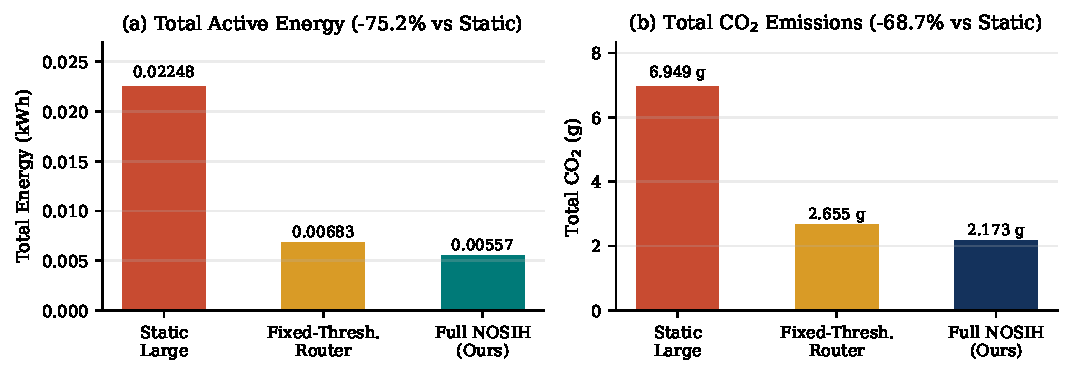
\includegraphics[width=0.96\linewidth]{figures/fig3_energy_carbon.pdf}
\caption{Active energy ($-75.2\%$ vs.\ Static; $-18.5\%$ vs.\ Fixed-Threshold) and operational $\text{CO}_2$ ($-68.7\%$ vs.\ Static) across the 240-prompt diurnal workload.}
\label{fig:ec}
\end{figure}

\begin{figure}[!t]
\centering
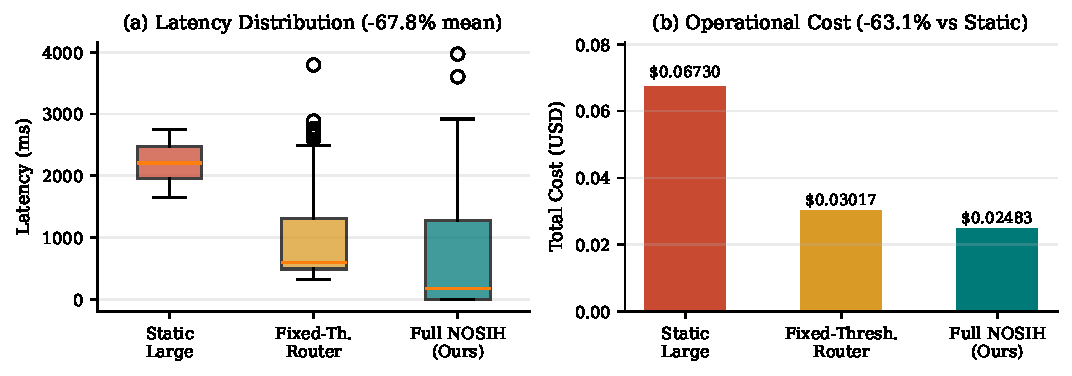
\includegraphics[width=0.96\linewidth]{figures/fig4_latency_cost.pdf}
\caption{(a) Latency distribution ($-67.8\%$ mean reduction vs.\ Static Large); (b) Operational cost comparison ($-63.1\%$ total reduction).}
\label{fig:lc}
\end{figure}

\begin{table}[!t]
\centering
\caption{NOSIH 5-Tier Routing Distribution ($n=240$ Queries)}
\label{tab:routing}
\scriptsize
\begin{tabular}{@{}lrr@{}}
\toprule
\textbf{Execution Tier} & \textbf{Queries} & \textbf{Share} \\
\midrule
$T_{0\text{a}}$: PS-RCSC Semantic Cache ($2.5\text{ W}$) & 64 & 26.7\% \\
$T_{0\text{b}}$: CPU Symbolic Ops ($4.5\text{ W}$) & 56 & 23.3\% \\
$T_1$: Small Neural 3B ($52\text{ W}$) & 35 & 14.6\% \\
$T_2$: Medium Neural 8B ($115\text{ W}$) & 50 & 20.8\% \\
$T_3$: Large Neural 32B ($175\text{ W}$) & 35 & 14.6\% \\
\midrule
\textbf{Total} & \textbf{240} & \textbf{100.0\%} \\
\bottomrule
\end{tabular}
\end{table}

\begin{figure}[!t]
\centering
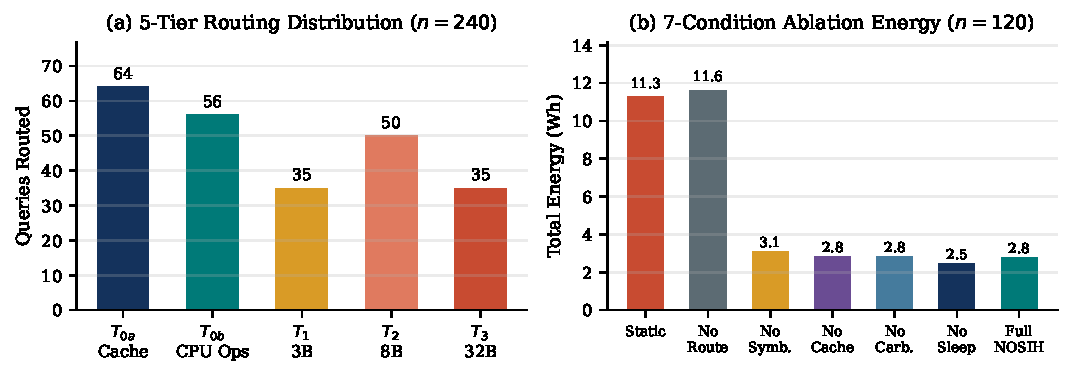
\includegraphics[width=0.96\linewidth]{figures/fig5_routing_power.pdf}
\caption{(a) 5-tier routing distribution ($n=240$); (b) 7-condition ablation active energy comparison ($n=120$).}
\label{fig:rp}
\end{figure}

\subsection{Ablation Study, Workload Scaling, and Async Concurrency}
Table~\ref{tab:ablation} isolates each subsystem across $n=120$ paired queries. Disabling dynamic routing (\texttt{Routing OFF}) increases active energy by $+3.0\%$ from $T_3$ wakeup overhead. Disabling symbolic offload (\texttt{Symbolic OFF}) drops task success from $96.67\%$ to $90.83\%$ and adds $+113.1\text{ ms}$ latency. Removing caching (\texttt{Cache OFF}) adds $+66.0\text{ ms}$, while disabling carbon duals raises $\text{CO}_2$ from $1.0679\text{ g}$ to $1.0990\text{ g}$. Removing sleep eliminates idle savings ($0.0\%$). Full NOSIH jointly achieves $-75.3\%$ active energy ($0.002779\text{ kWh}$), $-69.4\%$ $\text{CO}_2$, and $80.68\%$ idle power reduction.

Table~\ref{tab:scalability} verifies strictly linear workload energy scaling from $20$ to $240$ queries ($r = 0.9998$). To separate sequential workload scaling from runtime concurrency, we also physically benchmarked $C \in \{1, 10, 50, 100\}$ concurrent \texttt{asyncio} requests against \texttt{ZeroTrustKernel} with SQLite WAL: all $161/161$ completed with $0$ lock errors, scaling from $403.8\text{ req/s}$ ($C=1$, P95 $2.34\text{ ms}$) to $727.0\text{ req/s}$ ($C=100$, P50 $119.8\text{ ms}$, P95 $127.0\text{ ms}$, P99 $127.7\text{ ms}$); multi-GPU cluster scaling remains future work.

\begin{table}[!t]
\centering
\caption{7-Condition Ablation Study ($n=120$ Paired Queries)}
\label{tab:ablation}
\scriptsize
\begin{tabular}{@{}lccccc@{}}
\toprule
\textbf{Configuration} & \textbf{Lat.(ms)} & \textbf{Energy(kWh)} & $\boldsymbol{\Delta E}$ & $\boldsymbol{\Delta\text{CO}_2}$ & \textbf{Idle Cut} \\
\midrule
Static Large ($T_3$) & 2205.7 & 0.011267 & ref & ref & 0.00\% \\
Routing OFF & 2307.7 & 0.011607 & $+3.0\%$ & $+2.9\%$ & 72.17\% \\
Symbolic OFF & 823.0 & 0.003071 & $-72.7\%$ & $-66.6\%$ & 75.25\% \\
Cache OFF & 775.9 & 0.002821 & $-75.0\%$ & $-69.0\%$ & 78.40\% \\
Carbon Duals OFF & 712.4 & 0.002846 & $-74.7\%$ & $-68.5\%$ & 81.17\% \\
Sleep OFF & 613.9 & 0.002478 & $-78.0\%$ & $-72.5\%$ & 0.00\% \\
\textbf{Full NOSIH} & \textbf{709.9} & \textbf{0.002779} & \textbf{$-75.3\%$} & \textbf{$-69.4\%$} & \textbf{80.68\%} \\
\bottomrule
\end{tabular}
\end{table}

\begin{table}[!t]
\centering
\caption{Scalability Analysis: Linear Energy Scaling ($r = 0.9998$)}
\label{tab:scalability}
\scriptsize
\begin{tabular}{@{}rrrr@{}}
\toprule
\textbf{Queries} & \textbf{Avg Lat. (ms)} & \textbf{Total Energy (kWh)} & \textbf{Total $\text{CO}_2$ (g)} \\
\midrule
20 & 998.1 & 0.000553 & 0.1966 \\
60 & 752.6 & 0.001436 & 0.5411 \\
120 & 697.7 & 0.002740 & 1.0451 \\
240 & 707.6 & 0.005567 & 2.1728 \\
\bottomrule
\end{tabular}
\end{table}

\subsection{Zero-Trust Security, Races, and Conformal PID Behavior}
Table~\ref{tab:security} and Fig.~\ref{fig:sec} summarize Plane~I security and Plane~II conformal performance. Across a 100-case executable suite—30 benign operations and 70 attacks spanning 10 families (budget exhaustion, Base64/hex egress, duplicate-key differentials, multi-hop IPI, bank-master escalation, unallowlisted egress, Macaroon forgery, cache poisoning, cyclic/IFC DAGs, and rug pulls/Merkle tampering)—NOSIH attains $100.0\%$ benign utility ($30/30$, $0.0\%$ FPR, 95\% CI $[88.65\%, 100.0\%]$) and $100.0\%$ attack prevention ($70/70$, $0.0\%$ FNR, 95\% CI $[94.80\%, 100.0\%]$) at $<4\text{ ms}$ P95 proxy overhead ($2.47\text{ ms}$ mean). Under concurrency stress, SQLite WAL admits exactly $1/16$ in the 16-thread JTI race and $1/8$ in the 8-thread split-payout race. At $N=1{,}000$ leaves, \texttt{MTLog} verifies $10$-hash proofs in $<10\,\mu\text{s}$. All $46/46$ automated tests pass across 7 verification layers.

Across 5 seeds under post-shift overconfidence ($t \ge 500$, $T_{\text{post}}=800$), Conformal PID holds selective risk at $5.30\% \pm 0.12\%$ ($74.12\% \pm 1.17\%$ acceptance vs.\ $28.88\% \pm 1.41\%$ static error, $p=9.90\times 10^{-40}$). Because $5.30\%$ exceeds $\alpha=0.05$ by $+0.30\text{ pp}$ due to finite-sample integral lag ($O(1/(\eta T))$, Theorem~4), we do not claim a strict finite-sample $5\%$ bound: extending the horizon to $T_{\text{post}}=3000$ converges to $5.07\% \pm 0.02\%$, and setting a conservative target $\alpha_{\text{design}}=0.045$ holds finite-window risk at $4.72\% \pm 0.09\%$.

\begin{table}[!t]
\centering
\caption{Zero-Trust Security (100 Cases), Concurrency \& Conformal PID}
\label{tab:security}
\scriptsize
\begin{tabularx}{\linewidth}{lX}
\toprule
\textbf{Verification Metric} & \textbf{Measured NOSIH Result} \\
\midrule
Benign Utility / FPR & $30/30$ ($100.0\%$, $0.0\%$ FPR), CI $[88.65\%, 100.0\%]$ \\
Tool-Boundary APR / FNR & $70/70$ ($100.0\%$, $0.0\%$ FNR), CI $[94.80\%, 100.0\%]$ \\
Concurrency Races & $1/16$ JTI allowed; $1/8$ split-payout allowed \\
Proxy Overhead (CPU) & $<4\text{ ms}$ P95 ($2.47\text{ ms}$ mean) \\
Merkle Audit ($N=1{,}000$) & $10$ hashes ($<10\,\mu\text{s}$ inclusion \& consistency) \\
5-Seed Conformal PID & $5.30\% \pm 0.12\%$ risk ($74.12\%$ acc.\ vs.\ $28.88\%$ static) \\
Automated Test Suite & $46/46$ tests passed across 7 layers (0 failures) \\
\bottomrule
\end{tabularx}
\end{table}

\begin{figure}[!t]
\centering
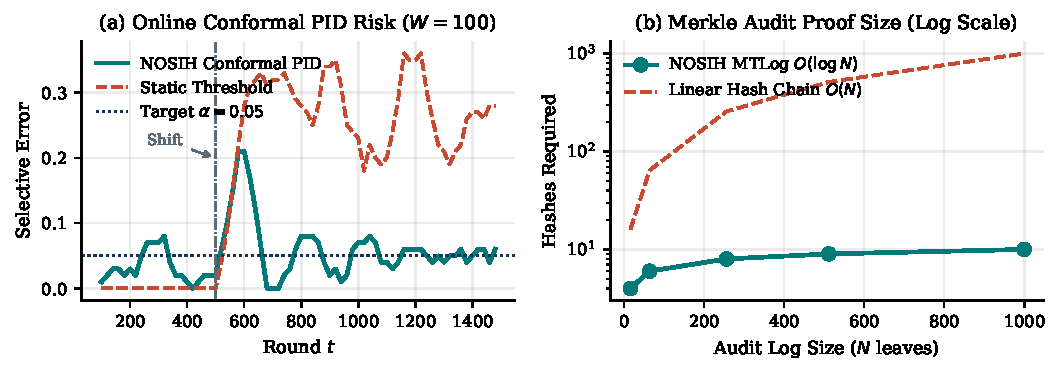
\includegraphics[width=0.96\linewidth]{figures/fig6_security_conformal.pdf}
\caption{(a) Online Conformal PID selective risk under shift ($5.30\% \pm 0.12\%$ vs.\ $28.88\%$ static, $p=9.90\times 10^{-40}$); (b) \texttt{MTLog} $O(\log N)$ proof scaling up to $N=1{,}000$ leaves ($10$ hashes).}
\label{fig:sec}
\end{figure}

\subsection{Cross-Plane Primitives: PCSP, PA-PCS-PMC, and CCEC}
Table~\ref{tab:novelty} and Fig.~\ref{fig:novelty} benchmark NOSIH's cross-plane primitives against decoupled baselines. Under $50$ peak-hour C-DoW prompts ($C(t)\in[450,515]\text{ gCO}_2/\text{kWh}$), a security-blind router consumes $4.5123\text{ Wh}$ and emits $2.1982\text{ g}$ $\text{CO}_2$, whereas PCSP mitigates $50/50$ attacks—cutting energy to $0.1415\text{ Wh}$ and $\text{CO}_2$ to $0.0689\text{ g}$ ($-96.9\%$). Under $40$ Sleep-Thrashing DoS probes targeting sleeping $T_3$ GPUs, reactive sleep wastes $7000.0\text{ J}$, whereas PA-PCS-PMC wastes $0.0\text{ J}$ ($-100.0\%$). Across $240$ Scope-2 CCEC receipts, $240/240$ verify in $7$ Merkle hashes, $20/20$ $\text{CO}_2$-tamper attempts are caught, and $20/20$ simulated-as-hardware spoofs are rejected.

\begin{table}[!t]
\centering
\caption{Cross-Plane Benchmark: PCSP, PA-PCS-PMC, and CCEC}
\label{tab:novelty}
\scriptsize
\begin{tabularx}{\linewidth}{lX}
\toprule
\textbf{Cross-Plane Primitive} & \textbf{Measured Result vs.\ Decoupled Baseline} \\
\midrule
PCSP vs.\ C-DoW ($n=50$) & $50/50$ mitigated; $0.0689\text{ g}$ vs.\ $2.1982\text{ g}$ $\text{CO}_2$ ($-96.9\%$) \\
PA-PCS-PMC Sleep-DoS ($n=40$) & $0.0\text{ J}$ vs.\ $7000.0\text{ J}$ wasted wakeups ($-100.0\%$) \\
CCEC Valid Receipts ($N=240$) & $240/240$ ($100.0\%$) verified in $7.93$ mean / $8$ max Merkle hashes \\
CCEC Tamper / Spoof & $20/20$ tampers caught; $20/20$ mode spoofs rejected \\
\bottomrule
\end{tabularx}
\end{table}

\begin{figure}[!t]
\centering
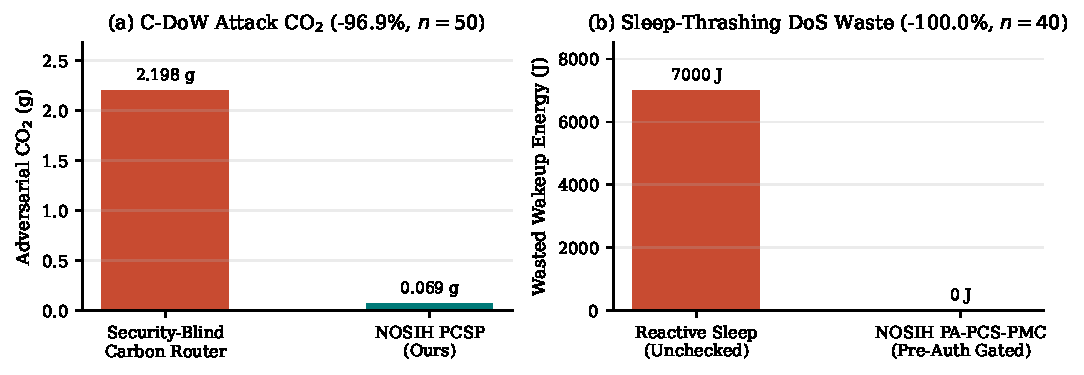
\includegraphics[width=0.96\linewidth]{figures/fig7_cross_plane_novelty.pdf}
\caption{(a) PCSP cuts C-DoW adversarial $\text{CO}_2$ by $96.9\%$ ($n=50$); (b) PA-PCS-PMC eliminates $100.0\%$ of Sleep-Thrashing DoS wakeup energy waste ($0.0\text{ J}$ vs.\ $7000.0\text{ J}$, $n=40$).}
\label{fig:novelty}
\end{figure}

\section{Discussion, Limitations, and Future Work}
Three operational lessons emerge from our evaluation. First, sustainability and accuracy reinforce one another: offloading deterministic arithmetic and policy lookups to $<5\text{ W}$ CPU engines cuts active energy by $75.2\%$ and cost by $63.1\%$ while lifting task success to $97.50\%$, lowering energy per successful goal by $75.3\%$. Second, EWMA hysteresis in PCS-PMC resolves the idle-burn vs.\ cold-start tradeoff, cutting GPU wakeups by $27.7\%$ ($68$ vs.\ $94$) and idle draw by $79.35\%$. Third, binding cache partitions, DAG capabilities, power wakeups, and linear budgets to a single provenance semiring blocks $70/70$ tool-boundary attacks at $<4\text{ ms}$ overhead while closing C-DoW and Sleep-Thrashing vectors.

\textbf{Deployment Integration \& Trade-Offs.} Integrating NOSIH into existing MCP deployments requires no changes to remote tool servers or LLM weights: operators supply an out-of-band signed tool manifest and configure tier power/cost metadata, while \texttt{ZeroTrustKernel} interposes at the JSON-RPC~2.0 boundary. Because Plane~I verification adds $<4\text{ ms}$ P95 overhead and Plane~II routing completes in $<15\,\mu\text{s}$, the dominant latency trade-off is the occasional $0.85\text{--}1.40\text{ s}$ \texttt{DEEP\_SLEEP} wakeup on infrequent $T_3$ bursts, which operators can bound by tightening the hysteresis multiplier $H_m$ for latency-critical tenants.

\textbf{Threats to Validity \& Future Work.} First, because our container lacks physical GPUs and NVML/RAPL counters, neural latency, accuracy, and GPU power rely on transparently tagged \texttt{CALIBRATED\_TRACE\_SIM}, \texttt{CALIBRATED\_BERNOULLI\_SIM}, and \texttt{HYBRID\_CPU\_TDP} models rather than hardware wattmeters (whereas all Plane~I security, WAL races, Merkle proofs, async concurrency, and 80 CPU symbolic queries are physically measured). Second, our 168-h carbon validation uses a synthetic diurnal+OU benchmark rather than live regional grid APIs. Third, our $0.0\%$ FNR applies strictly to tool-boundary authorization, provenance IFC, capability attenuation, cache isolation, and DAG execution; free-form prose manipulation that invokes no privileged tool lies outside the tool-boundary TCB. Future work will deploy NOSIH on multi-GPU Kubernetes clusters using \texttt{experiments/run\_hardware\_validation.py} with live NVML/RAPL counters and real-time grid carbon feeds.

\section{Conclusion}
We presented \textbf{NOSIH}, a Tri-Plane Closed-Loop Neuro-Symbolic Orchestration System unifying zero-trust MCP tool-boundary isolation (Plane~I), provenance-scoped caching, diurnal carbon-aware primal-dual routing, and online Conformal PID (Plane~II) with deterministic CPU engines, durable replay, and pre-authorized GPU power control (Plane~III). Across 240 diurnal queries and 100 security cases, NOSIH cuts active energy by $75.2\%$, $\text{CO}_2$ by $68.7\%$, cost by $63.1\%$, latency by $67.8\%$, and idle GPU power by $79.35\%$, outperforms a Fixed-Threshold Router by $18.5\%$ in energy and $18.2\%$ in $\text{CO}_2$, blocks $70/70$ tool-boundary attacks with $30/30$ benign utility, defeats C-DoW ($-96.9\%$ $\text{CO}_2$) and Sleep-Thrashing DoS ($-100.0\%$ waste), and passes $46/46$ automated tests.

\begin{thebibliography}{34}\scriptsize\setlength{\itemsep}{2.2pt}\setlength{\parskip}{0pt}
\bibitem{strubell2019energy} E. Strubell, A. Ganesh, and A. McCallum, ``Energy and policy considerations for deep learning in NLP,'' in \emph{Proc. ACL}, 2019, pp. 3645--3650.
\bibitem{schwartz2020greenai} R. Schwartz \emph{et al.}, ``Green AI,'' \emph{Commun. ACM}, vol. 63, no. 12, pp. 54--63, Dec. 2020.
\bibitem{patterson2021carbon} D. Patterson \emph{et al.}, ``Carbon emissions and large neural network training,'' \emph{arXiv:2104.10350}, 2021.
\bibitem{han2016deep} S. Han, H. Mao, and W. J. Dally, ``Deep compression,'' in \emph{Proc. ICLR}, 2016.
\bibitem{wu2024autogen} Q. Wu \emph{et al.}, ``AutoGen: Enabling next-gen LLM applications via multi-agent conversation,'' in \emph{Proc. COLM}, 2024.
\bibitem{hong2024metagpt} S. Hong \emph{et al.}, ``MetaGPT: Meta programming for a multi-agent collaborative framework,'' in \emph{Proc. ICLR}, 2024.
\bibitem{radovanovic2022carbon} A. Radovanovi\'c \emph{et al.}, ``Carbon-aware load balancing for geo-distributed cloud services,'' in \emph{Proc. ACM ASPLOS}, 2022, pp. 630--644.
\bibitem{wiesner2021wait} P. Wiesner, A. Trapp, and P. Leitner, ``Let's wait awhile: How temporal workload shifting can reduce carbon emissions in the cloud,'' in \emph{Proc. ACM/SPEC ICPE}, 2021, pp. 73--84.
\bibitem{li2025ecoserve} Y. Li \emph{et al.}, ``EcoServe: Designing carbon-aware AI inference systems,'' \emph{arXiv:2502.05043}, 2025.
\bibitem{tian2025greencache} J. Tian \emph{et al.}, ``GreenCache: Carbon-aware caching for LLM serving,'' \emph{arXiv:2505.23970}, 2025.
\bibitem{sheshanarayana2026gar} R. Sheshanarayana \emph{et al.}, ``GAR: Carbon-aware routing for LLM inference via constrained optimization,'' \emph{arXiv:2605.11603}, 2026.
\bibitem{carbonrouter2026} ``Context is not free: Carbon-aware LLM routing for multi-turn conversations,'' \emph{arXiv:2610.35230}, 2026.
\bibitem{patel2024power} P. Patel \emph{et al.}, ``Characterizing power management opportunities for LLMs in the cloud,'' in \emph{Proc. ACM ASPLOS}, 2024.
\bibitem{kakolyris2025throttllem} A. Kakolyris \emph{et al.}, ``throttLL'eM: SLO-aware GPU frequency scaling for energy efficient LLM inference serving,'' in \emph{Proc. IEEE HPCA}, 2025.
\bibitem{vllm2025sleep} vLLM Project, ``vLLM Sleep Mode Documentation,'' 2025.
\bibitem{wan2024neurosymbolic} Z. Wan \emph{et al.}, ``Towards efficient neuro-symbolic AI: From workload characterization to hardware architecture,'' \emph{IEEE TCASAI}, 2024.
\bibitem{chen2024frugalgpt} L. Chen, M. Zaharia, and J. Zou, ``FrugalGPT: How to use large language models while reducing cost and improving performance,'' \emph{TMLR}, 2024.
\bibitem{hu2024routerbench} Q. J. Hu \emph{et al.}, ``RouterBench: A benchmark for multi-LLM routing system,'' \emph{arXiv:2403.12031}, 2024.
\bibitem{ong2025routellm} I. Ong \emph{et al.}, ``RouteLLM: Learning to route LLMs with preference data,'' in \emph{Proc. ICLR}, 2025.
\bibitem{russac2019dlinucb} Y. Russac, C. Vernade, and O. Capp\'e, ``Weighted linear bandits for non-stationary environments,'' in \emph{Proc. NeurIPS}, 2019.
\bibitem{agrawal2016lincbwk} S. Agrawal and N. Devanur, ``Linear contextual bandits with knapsacks,'' in \emph{Proc. NeurIPS}, 2016.
\bibitem{angelopoulos2024crc} A. N. Angelopoulos \emph{et al.}, ``Conformal risk control,'' in \emph{Proc. ICLR}, 2024.
\bibitem{angelopoulos2023pid} A. N. Angelopoulos, E. Cand\`es, and R. J. Tibshirani, ``Conformal PID control for time series prediction,'' in \emph{Proc. NeurIPS}, 2023.
\bibitem{wu2026cachepoison} ``When cache poisoning meets LLM systems,'' in \emph{Proc. NDSS}, 2026.
\bibitem{debenedetti2025camel} E. Debenedetti \emph{et al.}, ``Defeating prompt injections by design (CaMeL),'' \emph{arXiv:2503.18813}, 2025.
\bibitem{costa2025fides} M. Costa \emph{et al.}, ``Securing AI agents with information-flow control (FIDES),'' \emph{arXiv:2505.23643}, 2025.
\bibitem{shi2025progent} T. Shi \emph{et al.}, ``Progent: Programmable privilege control for LLM agents,'' \emph{arXiv:2504.11703}, 2025.
\bibitem{wang2025mcptox} Z. Wang \emph{et al.}, ``MCPTox: A benchmark for tool poisoning attack on real-world MCP servers,'' \emph{arXiv:2508.14925}, 2025.
\bibitem{gaire2025sok} S. Gaire \emph{et al.}, ``SoK: Security and safety in the Model Context Protocol ecosystem,'' \emph{arXiv:2512.08290}, 2025.
\bibitem{rfc8785} A. Rundgren, B. Jordan, and S. Erdtman, ``JSON Canonicalization Scheme (JCS),'' IETF RFC 8785, 2020.
\bibitem{birgisson2014macaroons} A. Birgisson \emph{et al.}, ``Macaroons: Cookies with contextual caveats for decentralized authorization in the cloud,'' in \emph{Proc. NDSS}, 2014.
\bibitem{green2007semirings} T. J. Green, G. Karvounarakis, and V. Tannen, ``Provenance semirings,'' in \emph{Proc. ACM PODS}, 2007.
\bibitem{rfc6962} B. Laurie, A. Langley, and E. Kasper, ``Certificate Transparency,'' IETF RFC 6962, 2013.
\bibitem{rfc9162} B. Laurie \emph{et al.}, ``Certificate Transparency Version 2.0,'' IETF RFC 9162, 2021.
\end{thebibliography}

\end{document}
